\documentclass{article}
\usepackage{setspace}
\usepackage{geometry}
\usepackage[utf8]{inputenc}
\usepackage{amsmath,amsthm,amssymb}
\usepackage{mathtools}

\geometry{letterpaper, portrait, margin=1in}
\setstretch{1.5}
\title{Homework 1}
%\date{1-18-2020}
\author{Runmin Lu}

\begin{document}
	\maketitle
	%\newpage
	
	\section*{Exercise 1.3}
	\subsection*{(a)}
		Given that $\mathbf{x}(t)$ is misclassified by $\mathbf{w}(t)$, we know that $y(t) \neq \text{sign}(\mathbf{w}^T(t)\mathbf{x}(t))$. Either $y(t) > 0$ and $\mathbf{w}^T(t)\mathbf{x}(t) < 0$ or $y(t) < 0$ and $\mathbf{w}^T(t)\mathbf{x}(t) > 0$. Their product must be negative.
		
	\subsection*{(b)}
		\begin{align*}
			y(t)\mathbf{w}^T(t+1)\textbf{x}(t) &= y(t)(\mathbf{w}(t) + y(t)\mathbf x(t))^T\mathbf x(t)\\
			&= y(t)\mathbf{w}^T(t)\textbf{x}(t) + y(t)y(t)\mathbf x^T(t)\mathbf x(t)\\
			&= y(t)\mathbf{w}^T(t)\textbf{x}(t) + y(t)^2||\mathbf x(t)||^2\\
			&> y(t)\mathbf{w}^T(t)\textbf{x}(t)\\
			&\text{because } y(t)^2||\mathbf x(t)||^2 > 0 \text{ since } y(t) \neq 0, \mathbf x(t) \neq \mathbf 0
		\end{align*}
		
	\subsection*{(c)}
		In order to classify a datum correctly, we need $y(t)$ and $\mathbf{w}^T(t)\textbf{x}(t)$ to have the same sign. Equivalently, we want their product to be positive. After moving $\mathbf{w}(t)$ to $\mathbf{w}(t+1)$, we make the product greater, which is more positive, as shown in part (b).
		
	\section*{Exercise 1.5}
		(a) learning\\
		(b) design\\
		(c) learning\\
		(d) design\\
		(e) design
		
	\section*{Exercise 1.6}
	\subsection*{(a)}
		supervised\\
		input: each user's browsed books\\
		output: whether he/she read or ignored the books
	\subsection*{(b)}
		reinforcement\\
		input: games played against human\\
		some output: win/loss\\
		grade: win = +1, loss = -1
	\subsection*{(c)}
		supervised\\
		input: existing movies\\
		output: their classifications
	\subsection*{(d)}
		unsupervised\\
		input: existing music
	\subsection*{(e)}
		supervised\\
		input: existing customers\\
		output: their maximum debt
		
	\section*{Exercise 1.7}
	\subsection*{(a)}
		The hypothesis that always returns $\bullet$ gets picked.\\
		3 points: 1\\
		2 points: 3\\
		1 point: 3\\
		none: 1
		
	\subsection*{(b)}
		The hypothesis that always returns $\circ$ gets picked.\\
		3 points: 1\\
		2 points: 3\\
		1 point: 3\\
		none: 1
		
	\subsection*{(c)}
		$g(101) = \circ$\\
		$g(110) = \circ$\\
		$g(111) = \bullet$\\
		3 points: 1\\
		2 points: 3\\
		1 point: 3\\
		none: 1
		
	\subsection*{(d)}
		$g(101) = \bullet$\\
		$g(110) = \bullet$\\
		$g(111) = \circ$\\
		3 points: 1\\
		2 points: 3\\
		1 point: 3\\
		none: 1
		
	\section*{Problem 1.1}
		\begin{align*}
			P(\text{first black}) &= \frac34\\
			P(\text{two blacks}) &= \frac12\\
			P(\text{two blacks} | \text{first black}) &= \frac12 / \frac34\\
			&= \boxed{\frac23}
		\end{align*}
		
	\section*{Problem 1.2}
	\subsection*{(a)}
		\begin{align*}
			\text{What separates the region is represented by }\mathbf w^T\mathbf x &= 0\\
			\text{which is a line: } w_0 + w_1x_1 + w_2x_2 &= 0\\
			w_2x_2 = -w_1x_1 - w_0\\
			w_2 &= -\frac{w_1}{w_2}x_1 - \frac{w_0}{w_2}\\
			a &= -\frac{w_1}{w_2}\\
			b &= - \frac{w_0}{w_2}
		\end{align*}
	\subsection*{(b)}
		$\mathbf w = [1,2,3]^T$:\\
		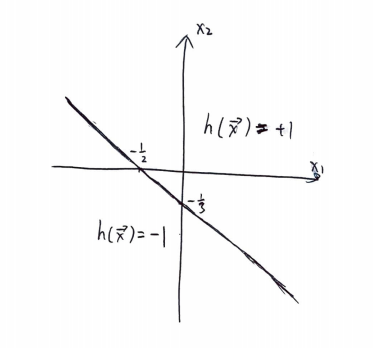
\includegraphics[scale=0.8]{p1.2b1.png}\\
		$\mathbf w = -[1,2,3]^T$:\\
		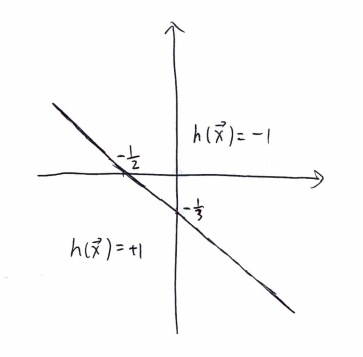
\includegraphics[scale=0.8]{p1.2b2.png}\\
		
	\section*{Problem 1.4}
	\subsection*{(a)}
		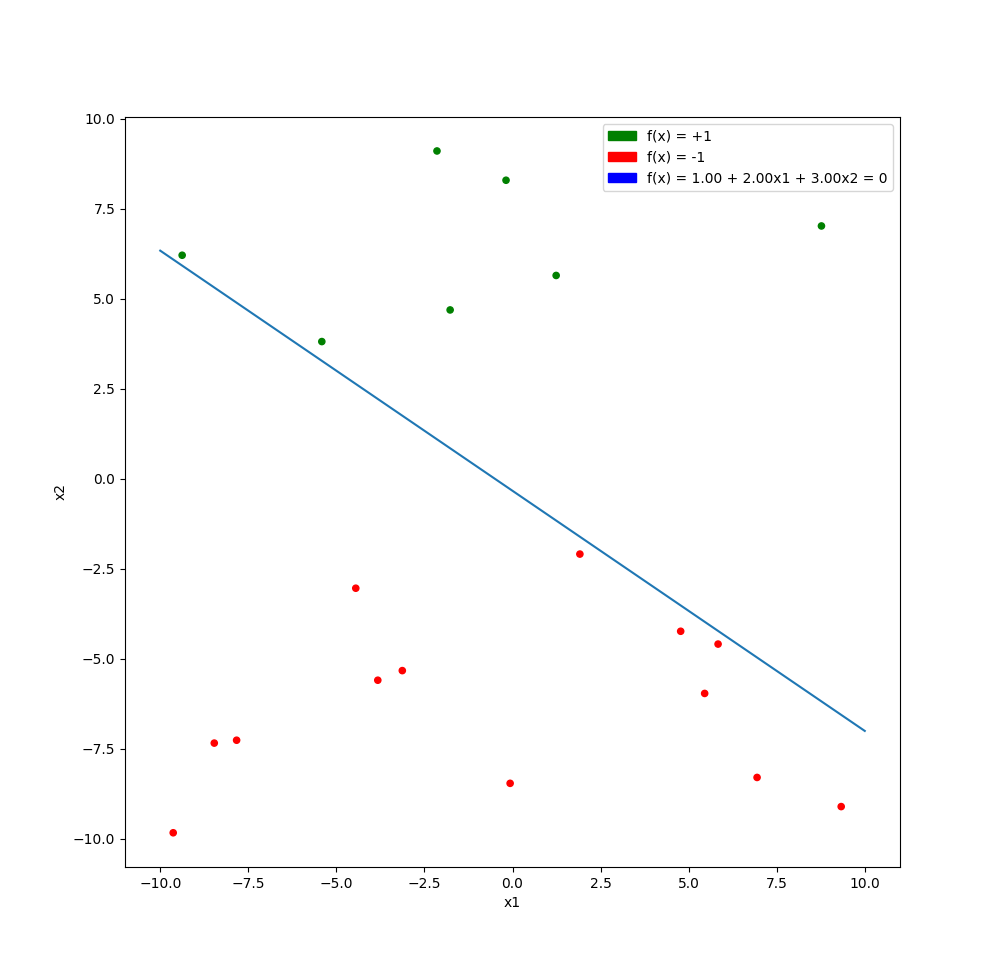
\includegraphics[scale=0.7]{p1.4a.png}
	\subsection*{(b)}
		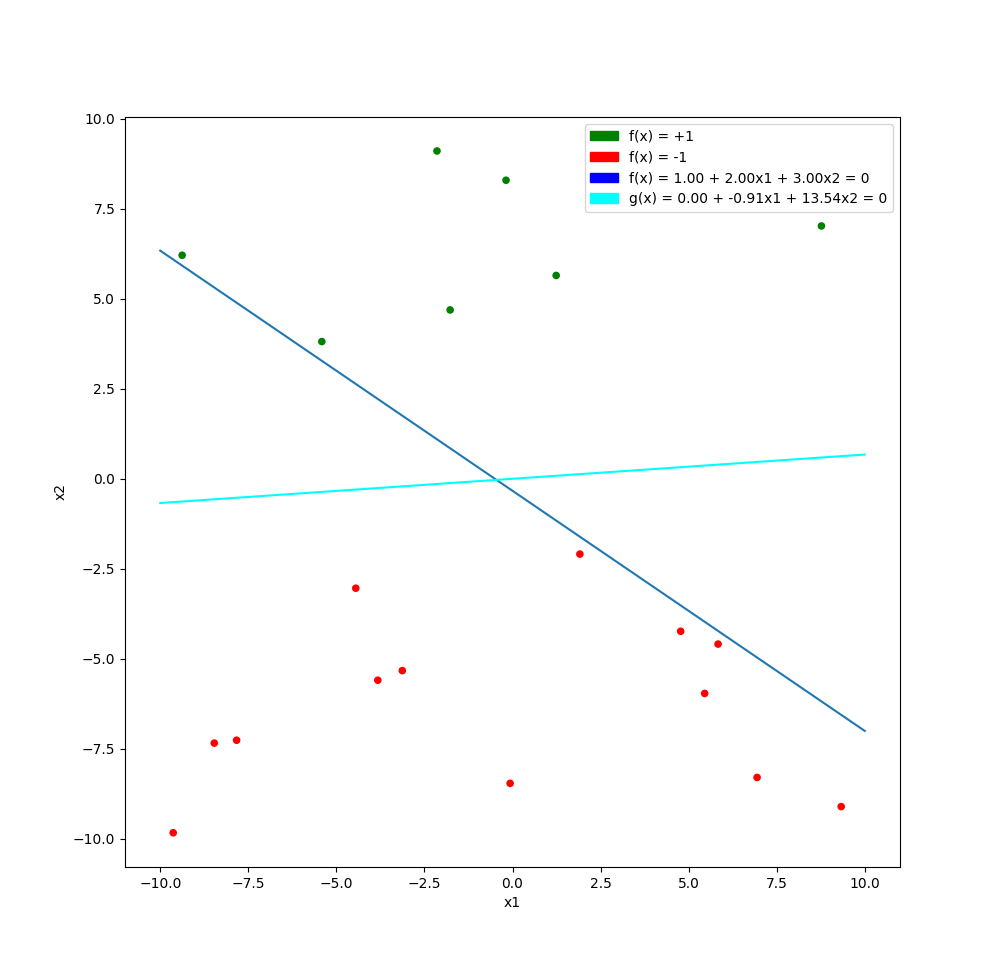
\includegraphics[scale=0.7]{p1.4b.png}\\
		$g$ is not close to $f$ at all because the size of the data is not large enough.
	\subsection*{(c)}
		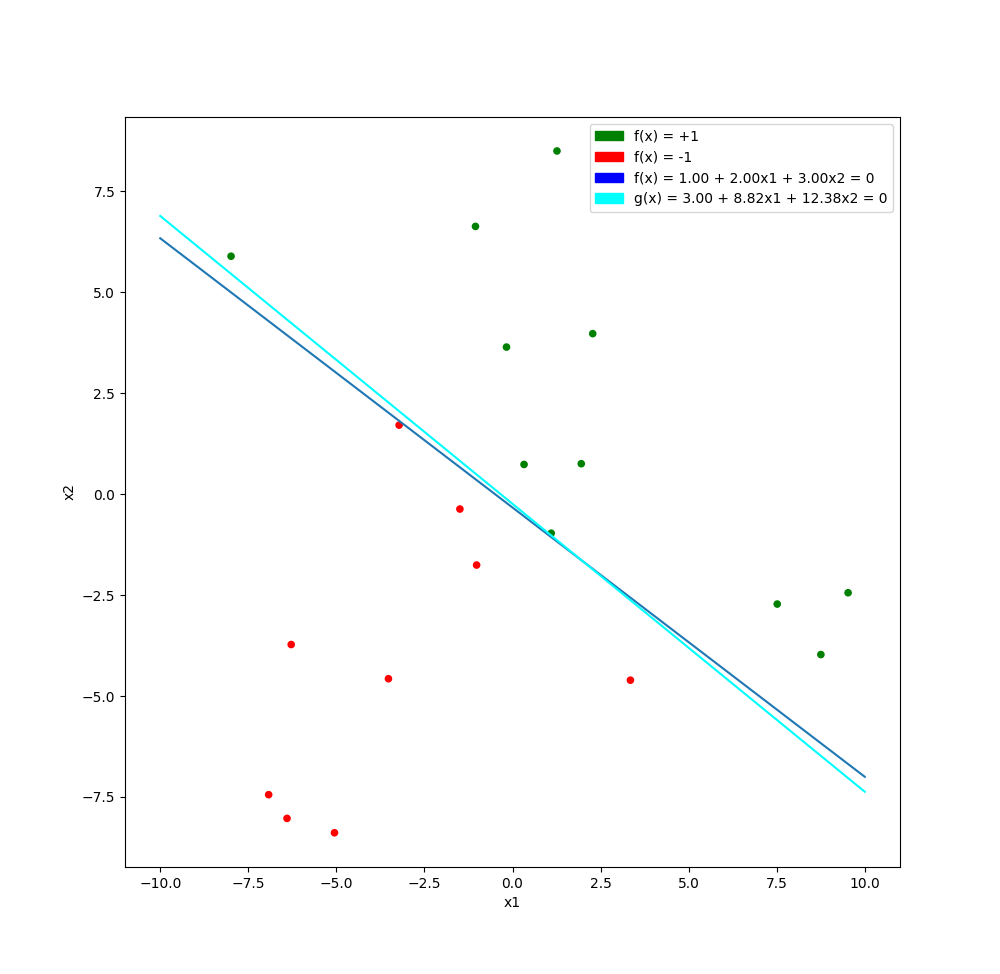
\includegraphics[scale=0.7]{p1.4c.png}\\
		This time $g$ is pretty close to $f$ because we got lucky that the data is better structured.
	\subsection*{(d)}
		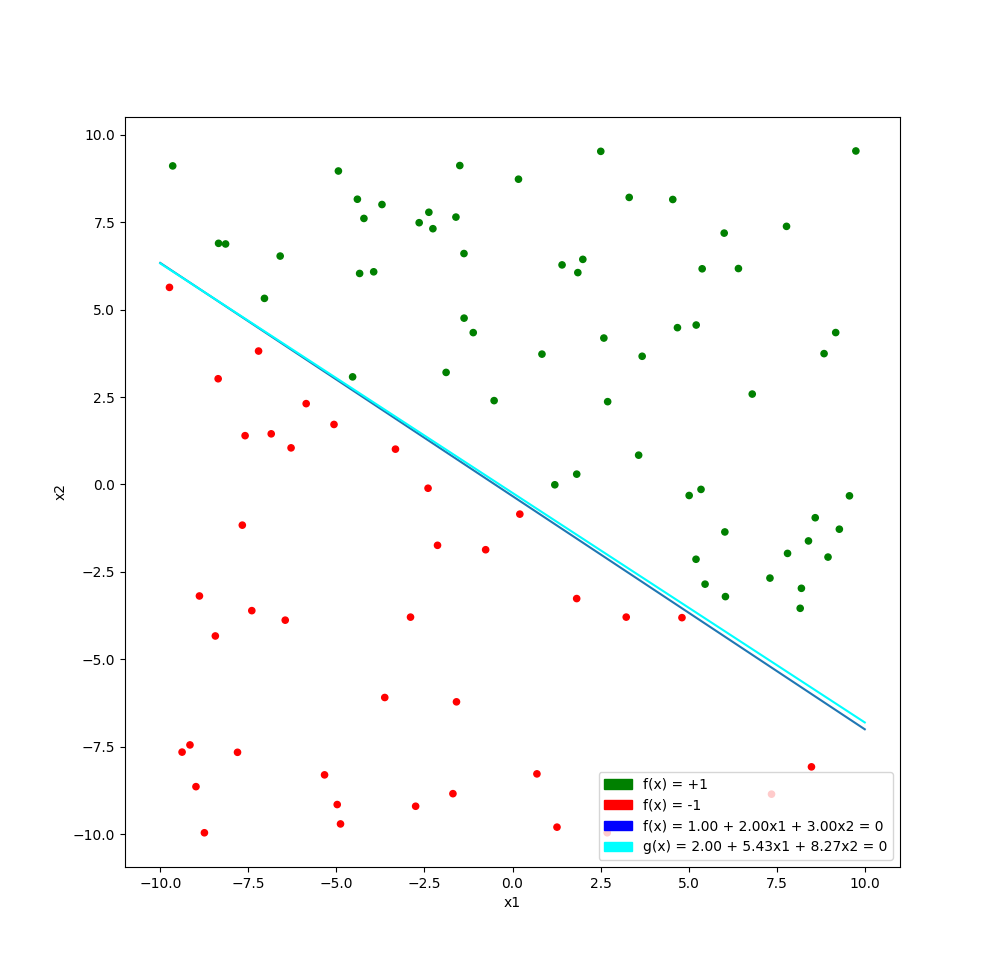
\includegraphics[scale=0.7]{p1.4d.png}\\
		$g$ is even closer to $f$ this time because the data size is much larger, which gives $g$ less freedom to move around without misclassifying any datum.
	\subsection*{(e)}
		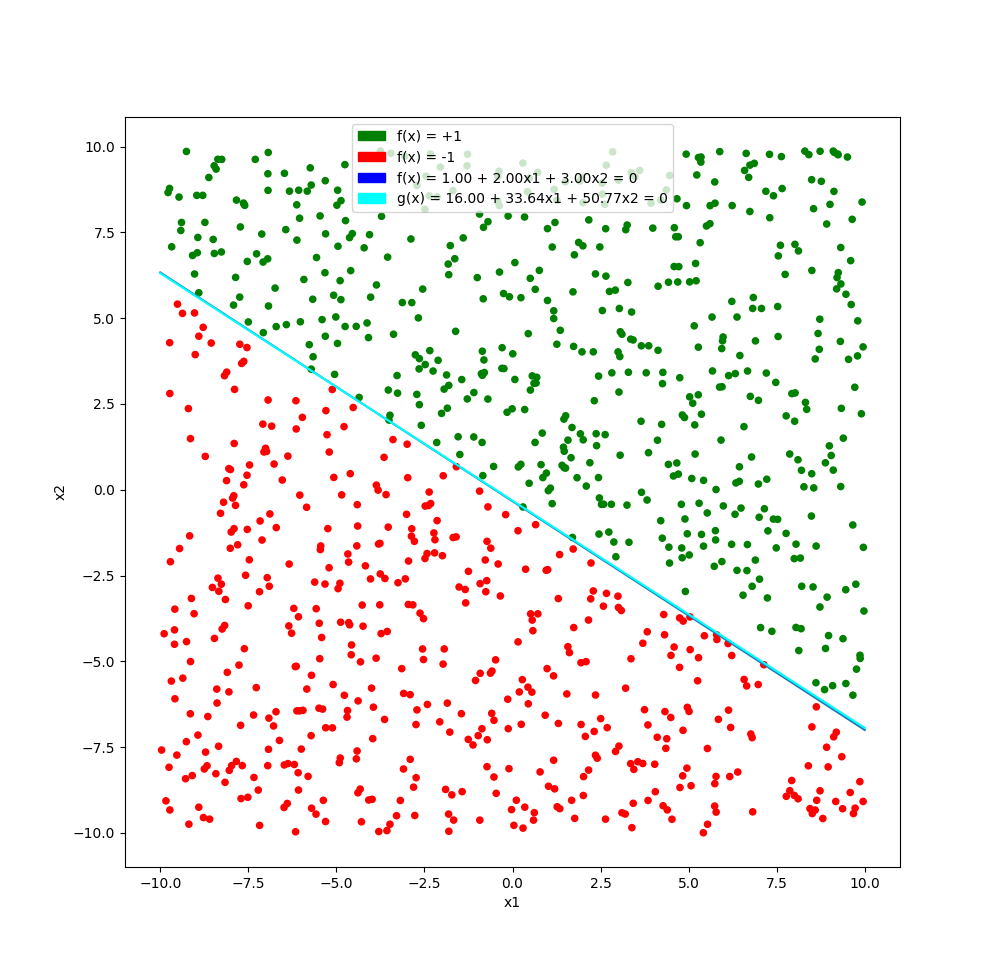
\includegraphics[scale=0.7]{p1.4e.png}\\
		In this case $g \approx f$ because the data size is even larger.
\end{document}